\subsection{Experimental Results}\label{sec:UAM-NFM-experiments}
In this section, we detail the results of a case study implementing the presented algorithm\footnote{The code for the implementation can be found at \url{https://github.com/JoeMuff999/Automata-Testing}}. All experiments were run on an AMD Ryzen 5 3600x processor with 6 cores @ 4.3 Ghz and 16 GB RAM. For the purposes of this demonstration, we use the prioritized safety specifications given in Example 3. We use the toolbox \textsc{TuLiP}~\cite{wongpiromsarn2011tulip} to compute minimally violating traces. 
We randomly generate vehicle requests in a format compatible with the Mission Planner Algorithm~\cite{guerreiro2019mission} developed at NASA Langley. The data contains simulated, timestamped on-demand requests for origin-destination trips corresponding to vertiports in particular vertihubs. We then run our algorithm to minimally violate the regulations described earlier.

\subsubsection{Scalability}
Figure~\ref{fig:runtime} shows the runtime per iteration per vertihub for different numbers of total vertihubs as well as the number of iterations until the algorithm converges. 
\begin{figure}[h!]
    \centering
    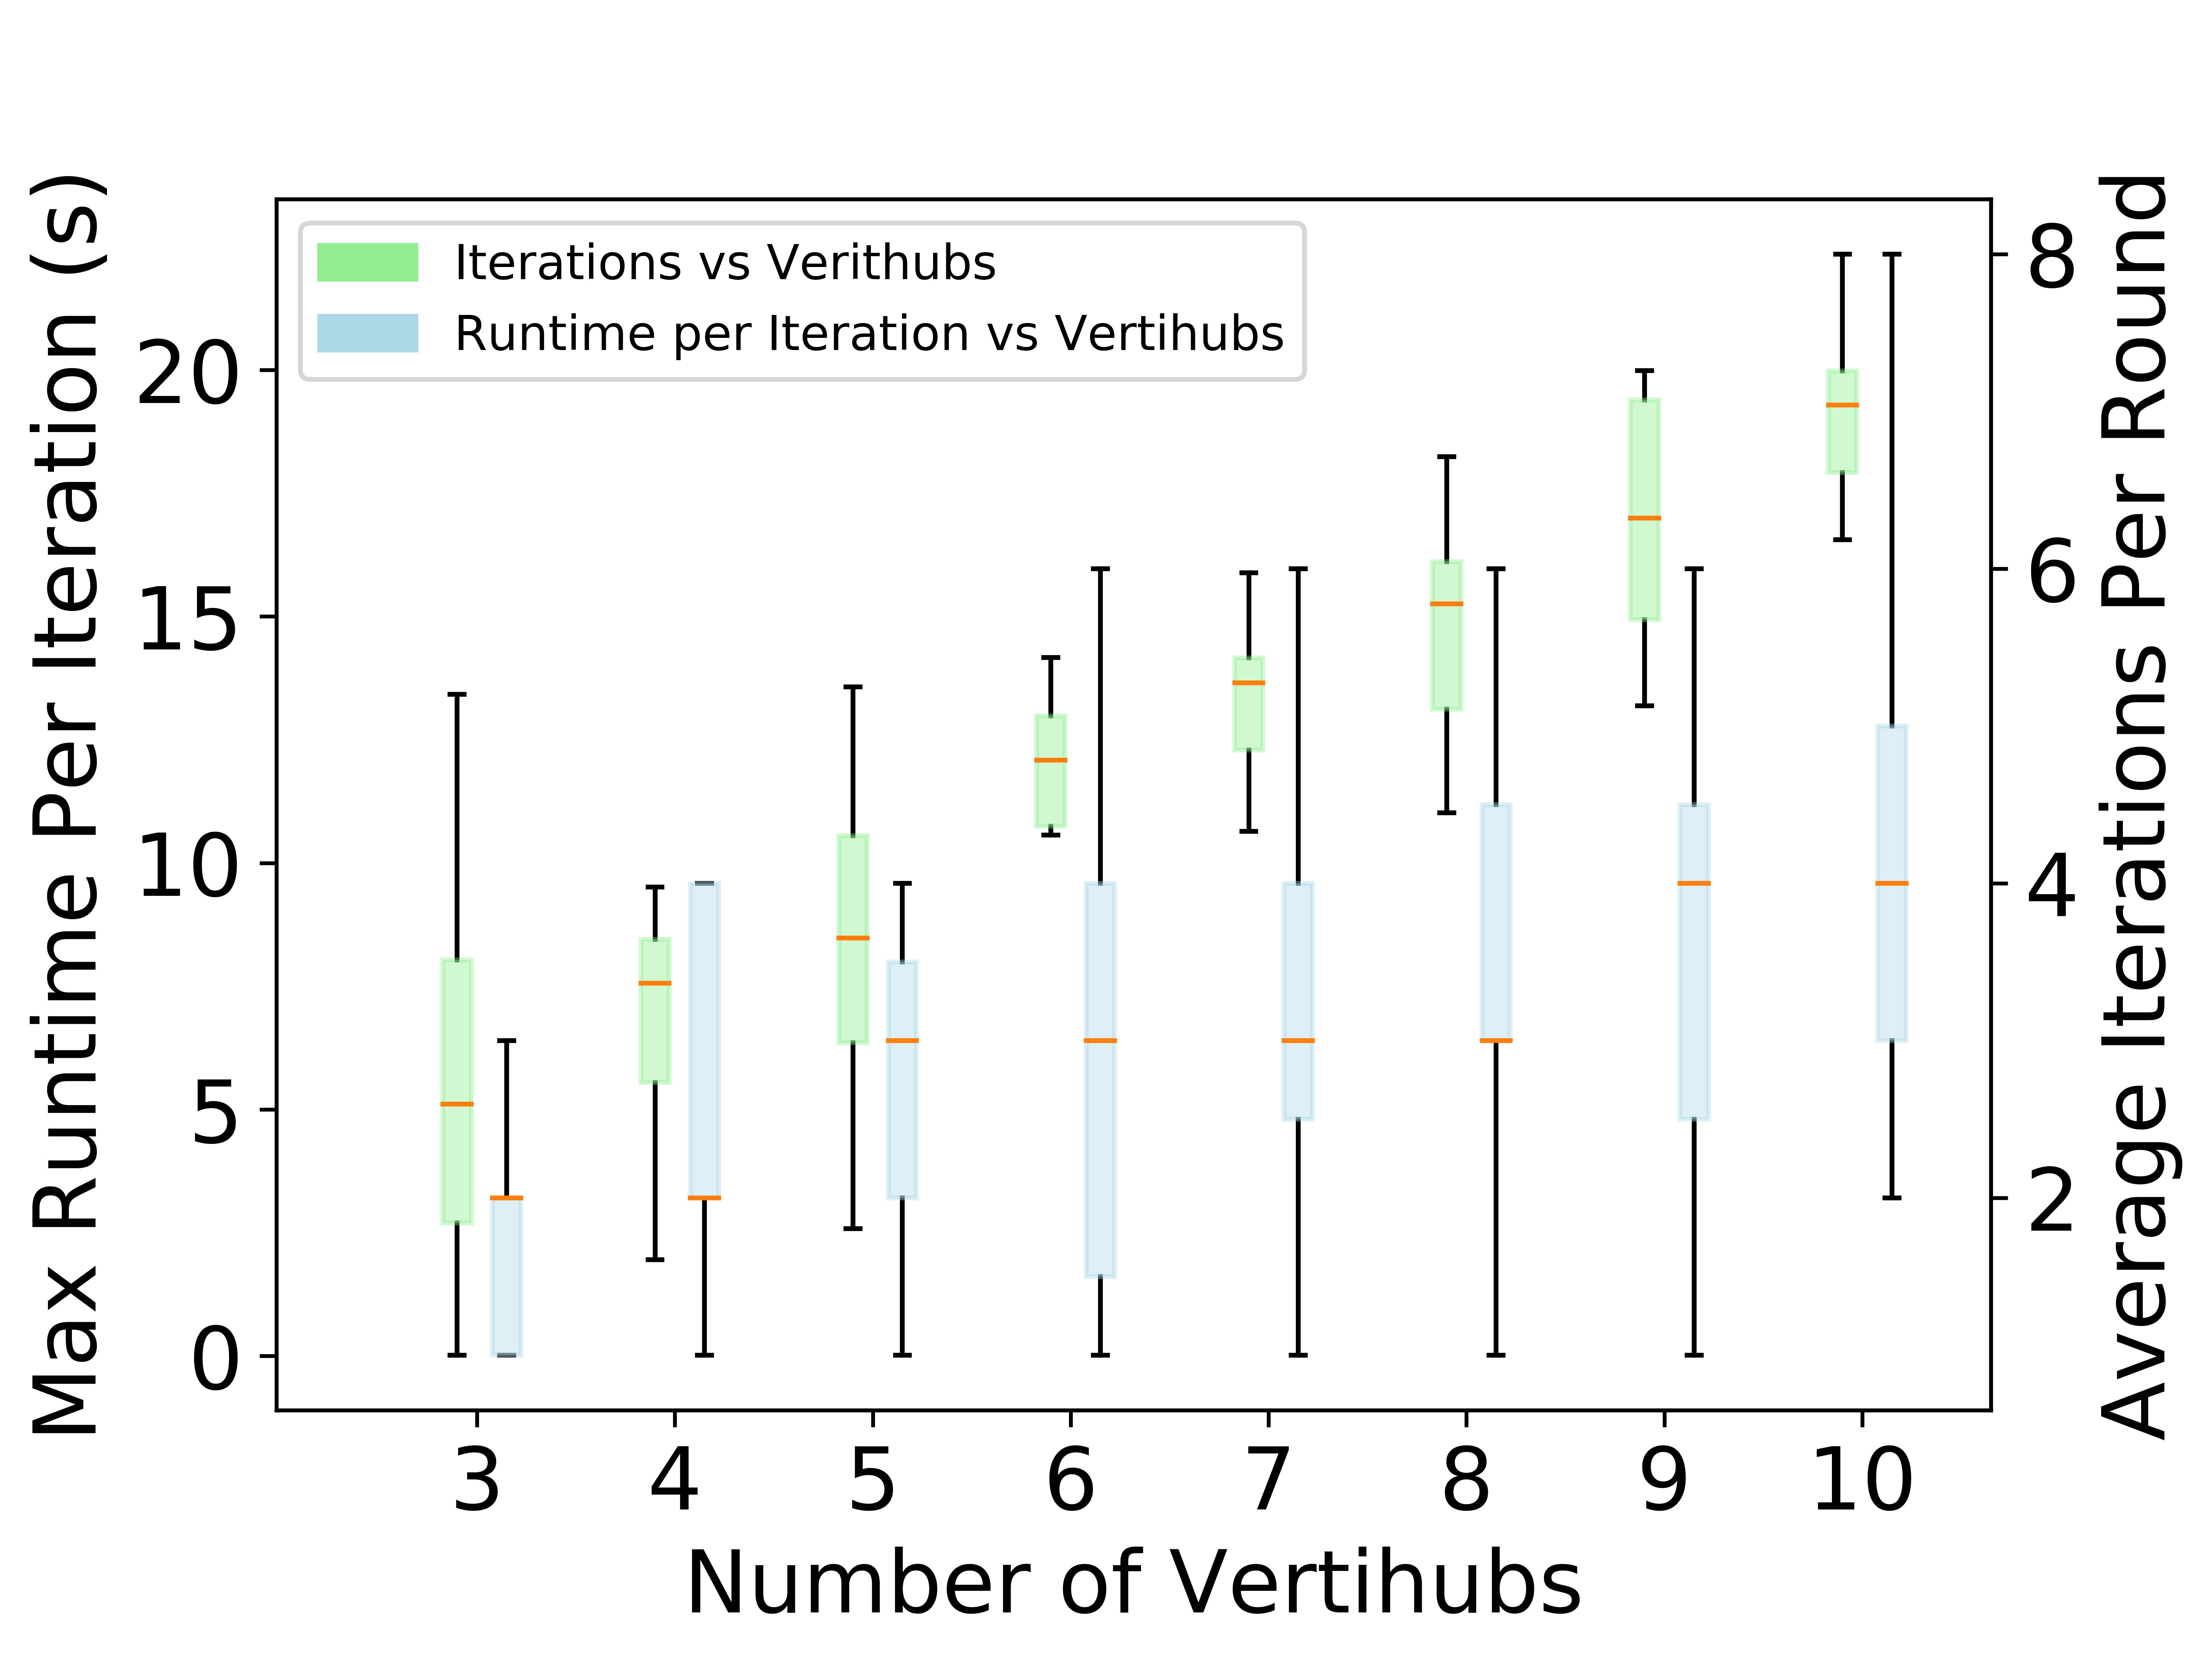
\includegraphics[width=0.8\columnwidth]{UAM-NFM/Figures/max_runtime_vs_size_boxplot_requests_static_with_iterations.png}
    \caption{Worst case runtime per iteration per vertihub (blue) and iterations until convergence (green).}
\label{fig:runtime}
\end{figure}
It is clear that the average runtime scales efficiently as the number of vertihubs increases.  In general, the total number of iterations before convergence also stays relatively constant albeit with a higher variance as the system size increases.  However, since the overall violation of the system's safety decreases with every iteration, in practice, we can always terminate the algorithm after a certain number of iterations and still have reduced the total violation cost. We note that even the smallest instance of the problem, i.e., 3 vertihubs with a maximum of 5 requests was unable to be solved in under 10 minutes using the centralized method. Furthermore, these results are a worst-case analysis as we assume the vertihubs are fully connected, i.e., all vertihubs can transfer requests to any other vertihub. In practice, the pool of vertihubs that can accept requests from other vertihubs will be smaller and this will limit the number of computations needed. 

\subsubsection{Violation cost}
To demonstrate the decreasing violation cost, we run our algorithm on the specific case of a 6 vertihub system with 10 requests. As shown in Figure~\ref{fig:costreduction}, the initial request allocation has a cost of 11 for the highest priority regulation. After 4 iterations, the cost has decreased to 0 while the cost for the second priority regulation stays at 2. 

\begin{figure}[h!]
    \centering
    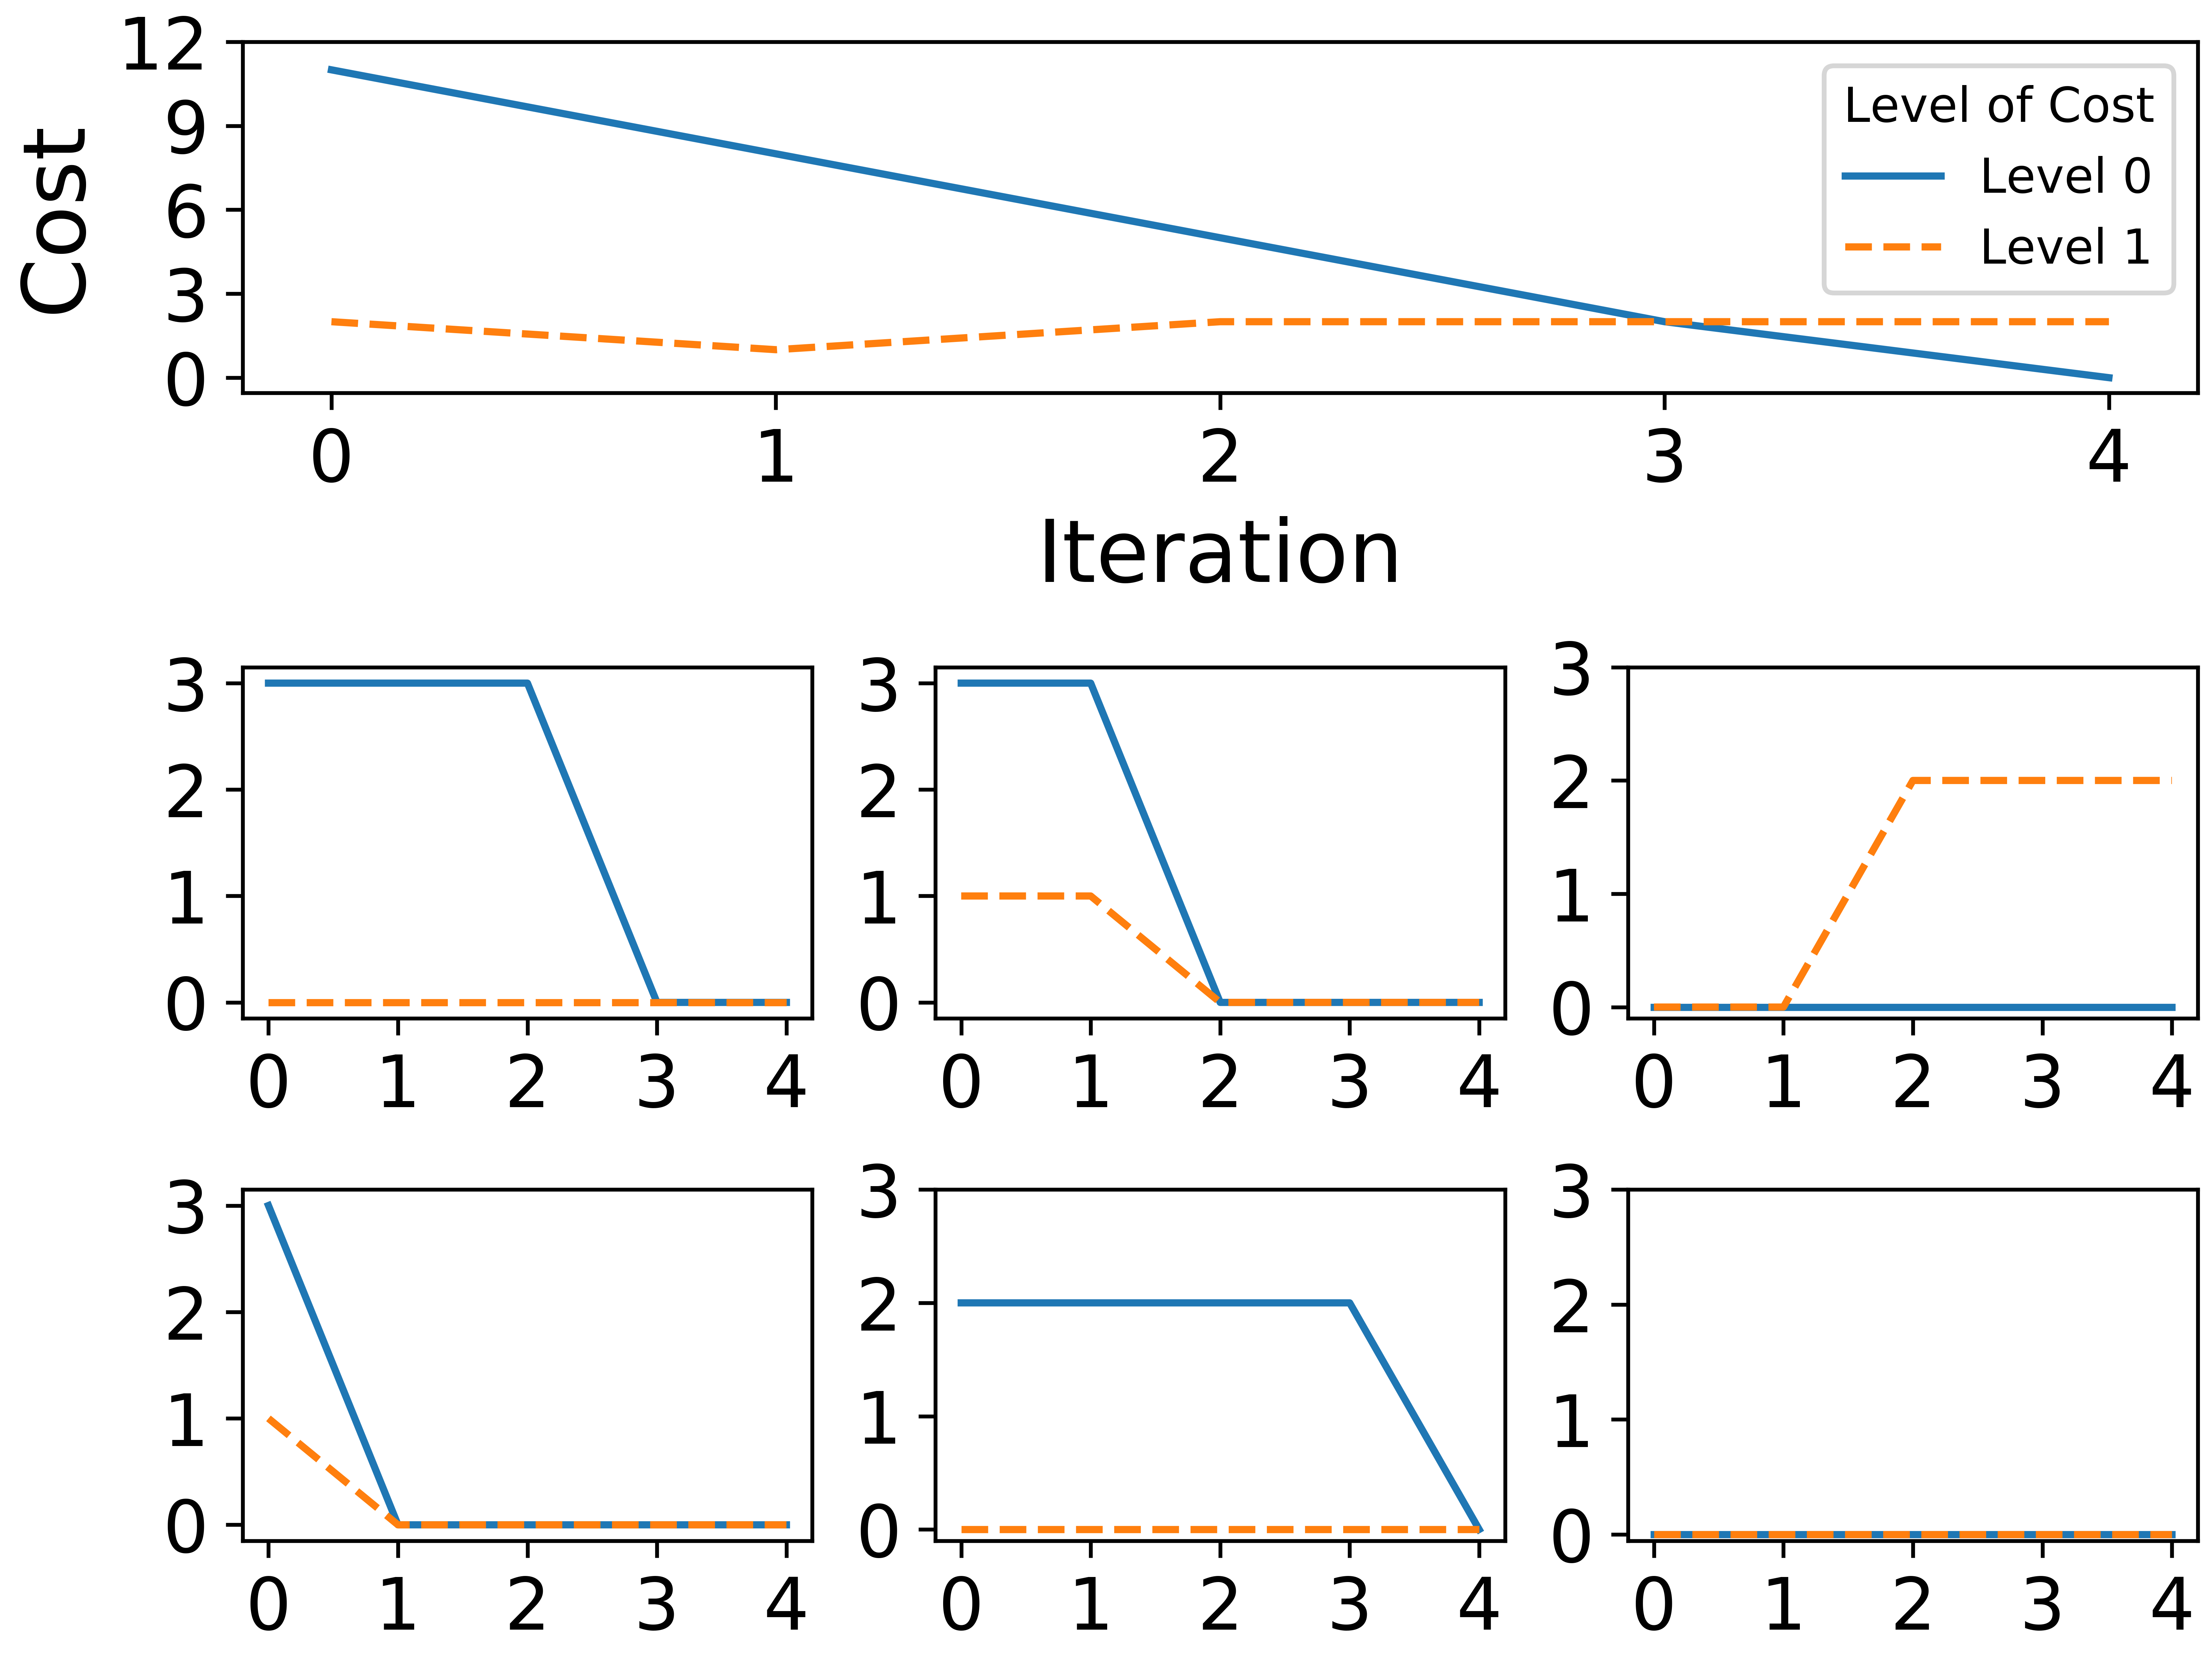
\includegraphics[width=0.85\columnwidth]{UAM-NFM/Figures/cost_vs_iteration_compiled.png}
    \caption{Violation cost vs iteration for a 6 vertihub system. Total violation, i.e., sum of the violation of all the individual vertihubs, is shown on top with the individual vertihub violation costs shown below.}
    \label{fig:costreduction}
\end{figure}



\subsubsection{Batch processing} The presented method in this section relies on processing batches of requests at a time. However, in practice, requests arrive sequentially in real time. In most cases however, the requests are known in advance and hence can be planned for. In this result, we demonstrate the effect of different batch sizes on overall violation cost. The data used in the simulation was generated by NASA Langley in conjunction with partners performing UAM demand studies. We divide incoming requests into batches of 5,10,and 15 requests at a time. Each batch is then processed before moving on to the next batch. We then sum the total violation cost across all batches for the entire data set. We note that we only report the level 1 violation cost as the level 0 violation cost is 0 in all cases. 

\begin{table}[]
\centering
\begin{tabular}{|c|c|c|} \toprule
Batch Size  & Violation Cost & Computation time (s) \\ \midrule
      5     &     71           &      6.6            \\
      10     &     63           &     32.5            \\
      15     &     56           &     161.9         \\ \bottomrule   
\end{tabular}
\caption{Level 1 violation cost and corresponding average synthesis time per batch per tower for different batch sizes.  } \label{tab:batchsizes}
\end{table}

As seen in Table~\ref{tab:batchsizes}, violation cost reduces as the batch size increases. This result is expected as the smaller batch sizes typically result in myopic plans that can cause violations down the road. However, it is not necessarily feasible to plan with large batch sizes as it requires a large look-ahead which may not be possible in practice. 

